\section{Results}
\label{sec:results}

Our experiments follow the logic of the introduction. We first establish how much of the context gain the band recovers and whether this finding is robust (Sec.~\ref{sec:dense_result}). We then test two explanations that would make the band unnecessary: that the same voxels would suffice if they entered the image network as sparse samples (Sec.~\ref{sec:source_result}), and that sparse samples would suffice if their geometry were read appropriately (Sec.~\ref{sec:spatial_result}). Finally, we ask which lesions benefit, which distinguishes lesion evidence from surrounding anatomy (Sec.~\ref{sec:anatomy_result}), and whether the effect carries over to other architectures (Sec.~\ref{sec:breadth_result}).

\begin{figure}[t]
  \centering
  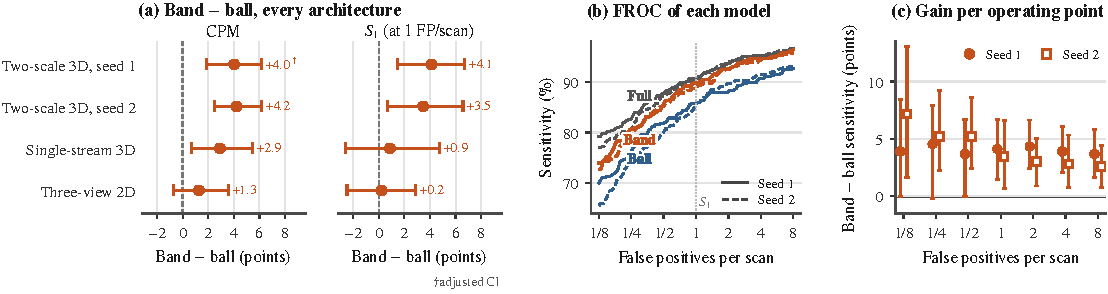
\includegraphics[width=\columnwidth]{figures/restoration.pdf}
  \caption{Restoring the band improves ranking. (a)~Band-minus-ball effects for every ranker ($^\dagger$adjusted interval). (b)~FROC curves of the two-scale ranker, seed~1 solid and seed~2 dashed. (c)~Band-minus-ball sensitivity at each CPM operating point.}
  \label{fig:restoration}
\end{figure}

\subsection{Effect of restoring the band}
\label{sec:dense_result}

With only the native ball visible, the two-scale ranker reaches \BallCpm\% CPM; adding the band raises it to \BandCpm\%, compared with \FullCpm\% for the full field (Tab.~\ref{tab:visibility}). The gain of \RestorePrimary{} points (adjusted interval) for seed~1 and \RestoreRepeat{} points for seed~2 corresponds to \PrimaryRecovery\% and \RepeatRecovery\% of the ball-to-full gap (Fig.~\ref{fig:restoration}a), and sensitivity at 1~FP/scan improves by \RestoreOne{} and \RepeatOne{} points. The point estimate is positive at all seven operating points for both seeds (Fig.~\ref{fig:restoration}b,c), while the full field retains an advantage of about 1.8 points.

\begin{figure}[t]
  \centering
  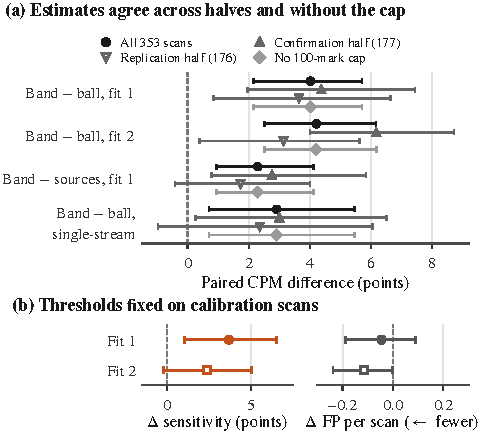
\includegraphics[width=\columnwidth]{figures/robustness.pdf}
  \caption{The band gain is robust. (a)~Effects on the whole pool, its two halves and without the 100-mark cap. (b)~Effects with thresholds fixed on the calibration set; seed~1 filled, seed~2 open.}
  \label{fig:robustness}
\end{figure}

These effects are stable across the two halves of the evaluation pool and unaffected by the 100-mark cap (Fig.~\ref{fig:robustness}a): the band-minus-ball gain lies between $+3.1$ and $+6.2$ points in every half, with intervals above zero for both seeds, and remains at $+4.03$ and $+4.21$ points without the cap. When thresholds are instead fixed in advance on the calibration set, sensitivity increases by $+3.69$ and $+2.39$ points, while the false-positive rate changes by less than $0.25$ per scan (Fig.~\ref{fig:robustness}b). Since the false-positive rate still differs slightly between models in this setting, we regard the matched comparisons as the primary evidence of improved ranking. Taken together, these results show that a thin shell of native CT, chosen only by the geometry of interpolation, carries most of the information that the full $32.4\mm$ field adds at fixed proposals.

\begin{table}[t]
\centering
\small
\setlength{\tabcolsep}{4.5pt}
\caption{Absolute CPM (\%) on the 353 evaluation scans for each visibility condition. Recovery is the share of the ball-to-full gap closed by the band. Paired effects with 95\% intervals are in Fig.~\ref{fig:restoration}a.}
\label{tab:visibility}
\begin{tabular}{@{}lrrrr@{}}
\toprule
Architecture & Ball & Ball+band & Full & Recovery \\
\midrule
Two-scale 3D, seed 1 & 83.58 & 87.60 & 89.37 & 70\% \\
Two-scale 3D, seed 2 & 82.83 & 87.05 & 88.63 & 73\% \\
Single-stream 3D & 80.94 & 83.85 & 85.84 & 59\% \\
Three-view 2D & 81.28 & 82.55 & 84.75 & 37\% \\
\bottomrule
\end{tabular}
\end{table}


\subsection{Coverage versus point of entry}
\label{sec:source_result}

\begin{figure}[t]
  \centering
  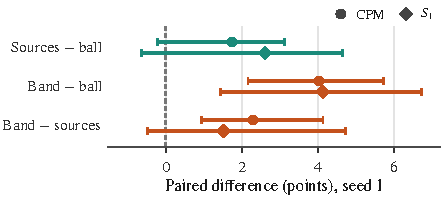
\includegraphics[width=\columnwidth]{figures/coverage.pdf}
  \caption{Dense coverage, not the point of entry, drives the gain: paired effects of native sources and band in the same two-scale network (seed~1).}
  \label{fig:coverage}
\end{figure}

A sparse head might underperform simply because its evidence arrives after the image features have been computed. The native-source condition removes this confound by providing the image network with every native voxel behind the 384 samples from the first convolution onwards. It nevertheless raises CPM over the ball by only \SourcesGain{} points, whereas the band adds a further \CoverageGap{} points over the native sources (Fig.~\ref{fig:coverage}). At 1~FP/scan, the corresponding effects ($+2.60$ and $+1.52$ points) have intervals that include zero, so the evidence is clearer for CPM than for any single operating point. Compared with the native sources, the band exposes 5.9 times as many exterior voxels (\BandSources{} versus \QuerySources{} per proposal) and forms a contiguous shell along which convolutional filters can follow structures. Since our intervention changes both properties together, it does not determine their relative contributions. What it does establish is that the advantage of the band is not an artefact of where its evidence enters the network.

\subsection{Sparse readouts and sample geometry}
\label{sec:spatial_result}

\begin{figure}[t]
  \centering
  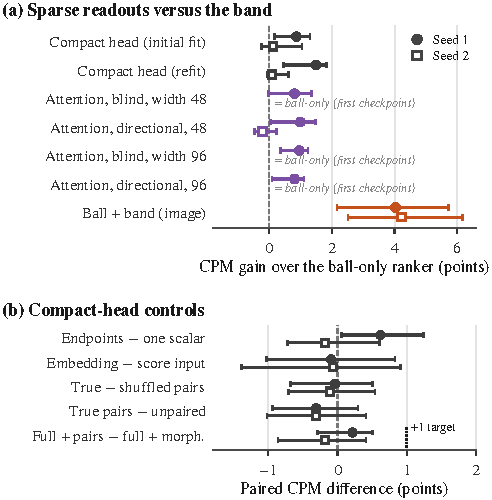
\includegraphics[width=\columnwidth]{figures/sparse.pdf}
  \caption{Sparse readouts remain far below the dense band. (a)~CPM gain of each readout over the ball-only ranker; italic notes mark seed-2 heads that kept their first checkpoint. (b)~Compact-head controls; the dotted mark is the $+1$ point target for the last row.}
  \label{fig:sparse}
\end{figure}

\begin{table}[t]
\centering
\small
\setlength{\tabcolsep}{4pt}
\caption{Absolute CPM and $S_1$ (\%) of every readout of the 384 sparse samples, with the image conditions for reference. $^\ast$Selected the first checkpoint; scores identical to the ball-only ranker.}
\label{tab:sparse}
\begin{tabular}{@{}lrrrr@{}}
\toprule
 & \multicolumn{2}{c}{Seed 1} & \multicolumn{2}{c}{Seed 2} \\
\cmidrule(lr){2-3}\cmidrule(l){4-5}
Readout & CPM & $S_1$ & CPM & $S_1$ \\
\midrule
Ball only (frozen) & 83.58 & 85.68 & 82.83 & 85.68 \\
Compact head, initial fit & 84.44 & 87.20 & 82.96 & 85.90 \\
Compact head, refit & 85.06 & 88.07 & 82.93 & 85.47 \\
Attention, blind, 48 & 84.38 & 86.98 & 82.83$^\ast$ & 85.68 \\
Attention, directional, 48 & 84.57 & 86.33 & 82.62 & 85.90 \\
Attention, blind, 96 & 84.54 & 87.42 & 82.83$^\ast$ & 85.68 \\
Attention, directional, 96 & 84.38 & 86.55 & 82.83$^\ast$ & 85.68 \\
\midrule
Dense band & 87.60 & 89.80 & 87.05 & 89.15 \\
Full field & 89.37 & 90.67 & 88.63 & 90.46 \\
\bottomrule
\end{tabular}
\end{table}


If the sparse samples underperformed only because pooling discards their relative directions, direction-aware attention should narrow the gap. For seed~1, all sparse heads improve on the ball-only ranker by 0.8--1.5 CPM points, but the difference between direction-aware and direction-blind attention is \GeometrySmallPrimary{} points at width 48 and \GeometryLargePrimary{} points at width 96 (Fig.~\ref{fig:sparse}a), and doubling the width brings no improvement. Tab.~\ref{tab:sparse} lists the absolute performance of every readout: the frozen ball-only ranker from which all heads start, the compact head in its initial fit and after refitting, the four attention heads, and, as references, the band and full-field image rankers. The best sparse readout, the refitted compact head, reaches 85.06\% CPM, compared with 87.60\% for the band; the band exceeds the compact refit by \CompactGapPrimary{} points and the direction-aware width-48 head by \ResidualSmallPrimary{} CPM points and \ResidualSmallOnePrimary{} points of $S_1$.

For seed~2, three of the four attention heads (direction-blind at both widths and direction-aware at width 96) retained their first checkpoint, whose output is identical to that of the ball-only ranker. Comparisons involving these heads are therefore comparisons with the ball-only ranker and carry no information about geometry. The remaining seed-2 heads change CPM by $-0.2$ to $+0.1$ points, and the band exceeds all of them by more than four points. Reading the samples more cleverly thus does not substitute for seeing the region they are drawn from. The compact-head controls in Fig.~\ref{fig:sparse}b are discussed in Sec.~\ref{sec:compact_result}.

\subsection{Where the gains occur}
\label{sec:anatomy_result}

\begin{figure}[t]
  \centering
  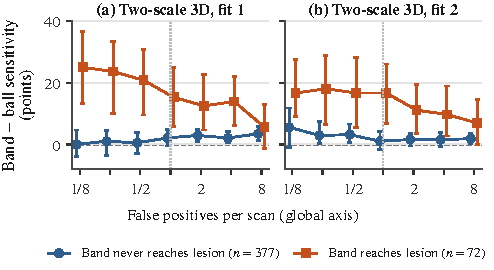
\includegraphics[width=\columnwidth]{figures/anatomy.pdf}
  \caption{The band helps most where it reaches the lesion. (a)~Share of lesions whose contour the band reaches, by diameter. (b,c)~Band-minus-ball sensitivity for reached ($n=72$) and never-reached ($n=377$) lesions.}
  \label{fig:anatomy}
\end{figure}

\begin{table}[t]
\centering
\small
\setlength{\tabcolsep}{3.5pt}
\caption{Sensitivity (\%) at a global 1 FP/scan by anatomy group, for the ball and band rankers. All 461 lesions stay in the global FROC. Diam.: median reference diameter (mm).}
\label{tab:anatomy}
\begin{tabular}{@{}lrrrrrr@{}}
\toprule
 & & & \multicolumn{2}{c}{Fit 1} & \multicolumn{2}{c}{Fit 2} \\
\cmidrule(lr){4-5}\cmidrule(l){6-7}
Group & $n$ & Diam. & Ball & Band & Ball & Band \\
\midrule
Reaches lesion & 72 & 17.4 & 69.4 & 84.7 & 69.4 & 86.1 \\
Never reaches & 377 & 5.8 & 89.9 & 92.0 & 89.9 & 91.0 \\
No contours & 6 & 6.0 & 100.0 & 100.0 & 100.0 & 100.0 \\
No proposal & 6 & 4.2 & 0.0 & 0.0 & 0.0 & 0.0 \\
\bottomrule
\end{tabular}
\end{table}


Among the 449 contoured lesions with a matching proposal, the band reaches \AnyOverlap{}, and whether it does is determined almost entirely by lesion size (Fig.~\ref{fig:anatomy}a): it reaches 70 of the 105 lesions of at least $10\mm$, 2 of the 137 lesions of 6--$10\mm$ and none of the 207 lesions below $6\mm$. At 1~FP/scan, restoring the band raises sensitivity on reached lesions by $+15.28$ and $+16.67$ points for the two seeds, compared with $+2.12$ and $+1.06$ points on the remaining \NeverOverlap{} lesions (Fig.~\ref{fig:anatomy}b,c); the between-group differences are $+13.16$ points $[3.68, 22.85]$ and $+15.61$ points $[4.69, 24.92]$. Tab.~\ref{tab:anatomy} gives the absolute sensitivities of all four lesion groups; the 6 lesions without usable contours and the 6 contoured lesions without a matching proposal remain in the global FROC but cannot be assigned to a reach group. Reached lesions are also those that the ball-only ranker handles worst: for seed~1, their sensitivity increases from 69.4\% to 84.7\%, whereas never-reached lesions improve from 89.9\% to 92.0\%. Roughly one sixth of the lesions thus account for more than half of the net gain at this operating point. For never-reached lesions, the gains at 8~FP/scan have intervals above zero for both seeds, whereas those at 1~FP/scan are compatible with small gains or small losses.

The two groups differ in more than band access. Reached lesions have a median reference diameter of $17.4\mm$, compared with $5.8\mm$, and more matching proposals; in addition, the grouping is observational, contour coverage is imperfect, and group sensitivities also depend on how false marks are ranked. We therefore conclude only that the largest gains occur where the restored voxels include annotated lesion tissue; how much patterns outside the lesion contribute remains open. A per-lesion analysis at the fixed seed-1 threshold agrees: the band gains 28 lesions and loses 9, and for 12 of the gained lesions the band of the highest-scoring mark reaches the contour (supplement Tab.~S19).

\subsection{Other architectures}
\label{sec:breadth_result}

The single-stream 3D network was retained because its full-field CPM exceeded 80\% on both the selection and the development set (\SingleCheck\% and \SingleDev\%), a criterion fixed in advance. On the evaluation pool, the band improves its CPM by \SingleGain{} points, recovering 59\% of its ball-to-full gap (Tab.~\ref{tab:visibility}), whereas its $S_1$ gain of $+0.87$ points is imprecise. The three-view 2D model gains \TriGain{} CPM points, which is inconclusive; since its views contain only a few central slices, the same 3D mask affects its input very differently. Rankers that process the full 3D field thus benefit from the band as well, while the evidence for slice-based inputs remains weak.

\subsection{Compact-head controls}
\label{sec:compact_result}

None of the design choices of the compact head has a consistent effect (Fig.~\ref{fig:sparse}b): every paired difference has an interval that includes zero, and the signs differ between seeds. Representing each axis by its two endpoints rather than a single scalar changes CPM by $+0.62$ and $-0.19$ points, using an image embedding instead of the image score changes the endpoint gain by $-0.09$ and $-0.06$ points, and preserving the true pairing of opposite half-axes changes CPM by $-0.03$ and $-0.11$ points relative to shuffled pairs and by $-0.31$ points for both seeds relative to unpaired half-axes. On a synthetic task in which pairing determines the label, the same heads reach 100\% accuracy, compared with 50\% for the shuffled and unpaired variants (supplement Sec.~S2), confirming that they can exploit pairing when it is informative.

Finally, we examine whether a sparse head remains useful once the full field is visible. Adding the paired head to the full-field ranker, compared against adding a grey-level morphology score of the band (the strongest such score on the development set; supplement Sec.~S3), changes CPM by \PracticalPrimary{} and \PracticalRepeat{} points. Both upper limits remain below $+1$ point, the smallest gain we had set in advance as practically relevant. At $1/8$~FP/scan, seed~1 stays within $-2$ sensitivity points of the full-field ranker, whereas the seed-2 interval extends below this margin. At fixed proposals, the benefit therefore comes from dense image access rather than from an additional readout.
